\section{Introduction}

This work investigates the non-resonant excitation of hexagonal Boron Nitride (hBN) defects at room temperature to achieve bright and pure single-photon emission. The aim is to fully characterise the emission, including spectrum, lifetime, brightness, purity and indistinguishability using a Hanbury Brown and Twiss (HBT) setup and a Michelson Interferometer. A complete characterisation of hBN emission at room temperature using these interferometry techniques has not been previously reported, and is critical for assessing the suitability of room-temperature hBN defect emission for quantum photonic platforms.

Efficient single-photon production is critical for advancing quantum photonic technologies, with applications including: enhancing measurement precision beyond classical limits \cite{Nagata2007, Vitelli2010} to enabling reliable transport and processing of analogue information in photonic circuits \cite{Bogaerts2020}. Among these applications, quantum key distribution (QKD) is the most mature, leveraging the quantum properties of single photons to detect eavesdropping attempts and create secure communication channels. 

The first QKD protocol proposed was BB84 \cite{Bennett2014}, in which Alice transmits photons polarised in one of two bases, the rectilinear basis ($\ket{H}$, $\ket{V}$) or the diagonal basis ($\ket{D}=(\ket{H}+\ket{V})/\sqrt{2}$, $\ket{A}=(\ket{H}-\ket{V})/\sqrt{2}$), to encode binary bits in two mutually unbiased bases. Bob randomly selects a basis for each measurement and publicly announces which basis was used, retaining only results where their basis choices match to construct a shared secret key. An eavesdropper (Eve) intercepting a photon must randomly pick a basis when sending on the next photon, with a $\frac{1}{2}$ chance of error, collapsing the state and introducing detectable discrepancies when she resends the photon. The probability of Eve correctly guessing all $n$ bases by chance is $\left(\frac{1}{2}\right)^n$, decreasing exponentially with $n$ and allowing security to be arbitrarily strengthened. Although BB84 is provably secure in ideal quantum settings \cite{Shor2000}, practical implementations using attenuated laser pulses instead of true single-photon sources are vulnerable to photon-number splitting (PNS) attacks \cite{Ashkenazy2024}, where Eve uses a beam splitter to extract information without inducing detectable errors, thereby imposing a theoretical upper-limit on the secure key rate (SKR). This limitation has been overcome experimentally with single-photon sources, which have surpassed the SKR achievable with attenuated lasers \cite{Zhang2025}.


This thesis is ordered in the following way. The remainder of Section 1 introduces the fundamental concepts relevant to single-photon emitters: initially section 1.1 provides an overview of the defining characteristics used to evaluate their performance, such as purity, brightness, and indistinguishability. Followed by section 1.3 which introduces hBN as a promising platform for hosting single-photon emitters. Section 2 then details the experimental setup and techniques used throughout this study to investigate the emission from hBN defects. Finally, Section 3 presents the key experimental results, including measurements of single-photon purity, brightness, and photon indistinguishability for a specific hBN defect emitter.

\subsection{Benchmarking Single-Photon Sources}

An ideal single-photon source should emit exactly one photon on demand, with each photon possessing identical characteristics. To assess the quality of a single-photon source, three key parameters are evaluated: Purity ($P$), Indistinguishability ($I$), and Brightness ($B$). For an ideal source, all three parameters reach their maximum value, such that $ P = I = B = 1 $.

\begin{figure}[h]
    \centering
    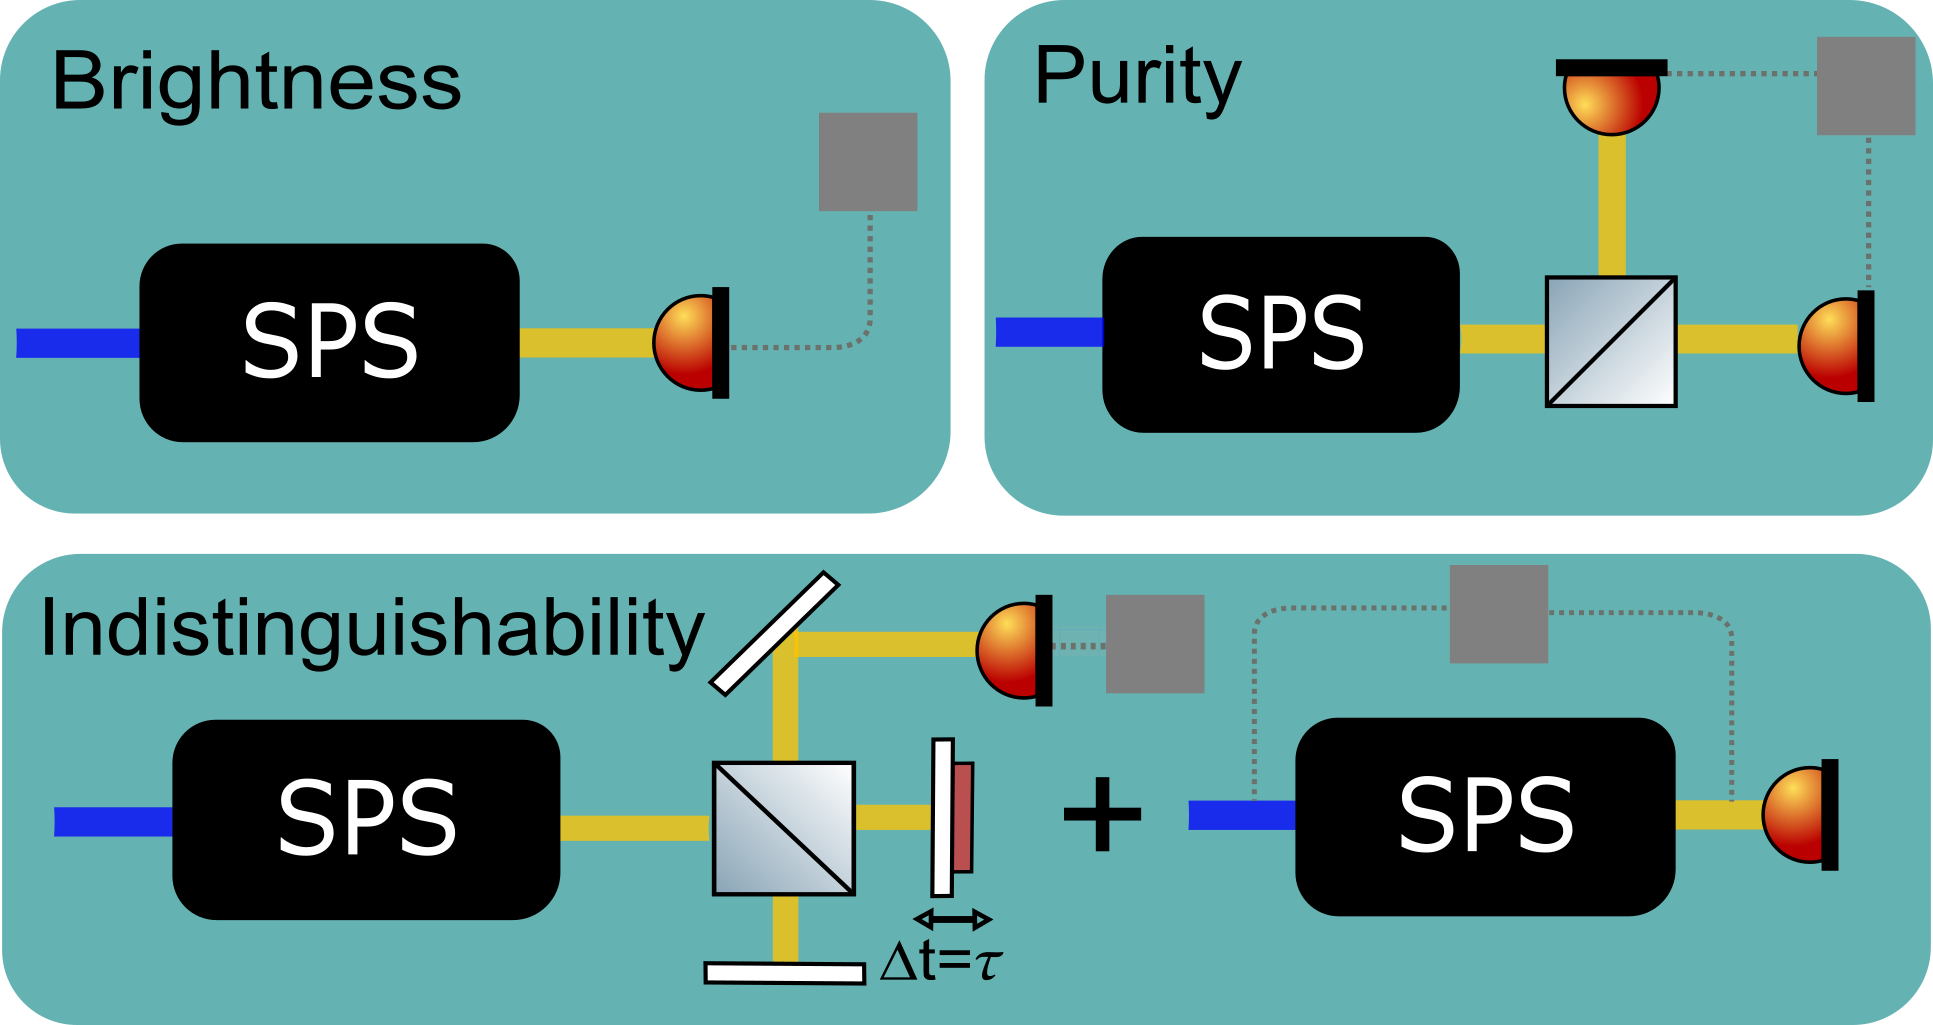
\includegraphics[width=0.9\linewidth]{Figures/PIB.png}
    \caption{Schematic of the respective setups used to measure brightness, purity and indistinguishability. Brightness is measured directly using a photon detector, while purity is measured using a HBT interferometer. To calculate indistinguishability, a Michelson interferometer is used to measure the pure dephasing rate, and a separate lifetime measurement is needed to calculate the total dephasing rate. The grey boxes are a photon counting/correlating device.}
    \label{fig:PIB}
\end{figure}

\subsubsection{Brightness}

The brightness describes the probability that a single photon is emitted per excitation pulse. Unlike $P$ and $I$, brightness is a loss-dependent measure, as it depends on the detection efficiency and optical setup. Therefore, when comparing sources, it is important to distinguish between the brightness at the source ($B_s$), measured before any optical losses, and the detected brightness ($B_d$), which is affected by transmission losses, collection and detector efficiency. This measurement is performed directly using a photon detector, Fig.~\ref{fig:PIB}.

\subsubsection{\label{sec:purity} Purity}
Purity is a loss-independent measure that quantifies the likelihood that the source emits only one photon at a time. It is defined as $P = 1 - g^{(2)}(0)$, where $g^{(2)}(0)$ is the second-order correlation function at zero time delay. The function $g^{(2)}(\tau)$ describes the statistical correlation between detecting two photons separated by a time delay $\tau$ relative to a completely random (Poissonian) photon distribution:

\begin{equation}
    g^{(2)}(\tau) = \frac{\langle I(t)I(t+\tau)\rangle}{\langle I(t)\rangle^2},
    \label{eqn:g2}
\end{equation}

where $\langle \rangle$ denotes a time-averaged quantity, and $I(t)$ is the measured photon intensity at time $t$. For an ideal single-photon emitter, $g^{(2)}(0) = 0$ indicates perfect antibunching, meaning photons are emitted strictly one at a time without multi-photon events, while coherent light from a laser has $g^{(2)}(0) = 1$, reflecting Poissonian statistics and uncorrelated detections. In contrast, thermal sources exhibit $g^{(2)}(0) > 1$, characteristic of photon bunching due to bosonic effects. Practically, achieving $g^{(2)}(0) \ll 0.5$ strongly suggests a non-classical light source capable of single-photon emission, typically measured using a Hanbury Brown and Twiss (HBT) interferometer \cite{Brown1956}, as shown in Fig.~\ref{fig:PIB}.


The HBT interferometer was originally developed to measure the angular size of stars \cite{HanburyBrown1956} by correlating the intensity fluctuations between between two detectors. Unlike most interferometry, it does not rely on interference but rather on correlations in photon arrival times. To measure $g^{(2)}(\tau)$ using the HBT setup, the photon detection's at one detector and the subsequent event's at the other are recorded over an extended time. The delays are then plotted for all detection events, and the value of $g^{(2)}(0)$ can be extracted.


\subsubsection{Indistinguishability}

Indistinguishability, a loss-independent measure, quantifies the probability that two photons will interfere in a Hong-Ou-Mandel (HOM) setup \cite{Hong1987}, where two indistinguishable photons arriving simultaneously at a 50:50 beam splitter always exit through the same output port, a phenomenon essential to quantum photonic applications relying on entanglement \cite{Kok2007, Knill2001}.

For photons to be indistinguishable, they must share the same spatial mode, spectral and temporal profiles, and phase state \cite{Senellart2017}. Spatial mode alignment is typically achieved using single-mode fibres, while the spectral and temporal characteristics depend on the emitter’s linewidth $\Gamma/2\pi$ and spontaneous decay rate $\frac{1}{T_1}=\gamma/2\pi$, respectively. Phase coherence is determined by the pure dephasing rate $\frac{1}{T_2^*}=\gamma^*/2\pi$, measurable with a Michelson interferometer \cite{Michelson1887, Jelezko2003}. The Michelson interferometer, first developed to study the properties of light \cite{Michelson1887}, splits an incoming light beam into two paths using a beam splitter. By introducing a difference in path length to one of the arms, one of the beams is delayed temporally, and the recombined beam produces an interference pattern which can be used to measure the optical properties of the source.

Indistinguishability can be calculated via $g^{(2)}_{\text{HOM}}(0)$ measured in a path-unbalanced Mach-Zehnder interferometer using sequential single-photons, where perfect indistinguishability yields $g^{(2)}_{\text{HOM}}(0)=0$ and $I=1-2g^{(2)}_{\text{HOM}}(0)$. However, in this work, indistinguishability is determined by extracting the emitter’s pure dephasing rate with a Michelson interferometer and its radiative lifetime via time-resolved photoluminescence (PL) measurements, Fig.~\ref{fig:PIB}, yielding $I=\frac{\gamma}{\Gamma}=\frac{\gamma}{\gamma+2\gamma^*}$.

\subsection{Types of Single-photon Source}

\subsubsection{Probabilistic Single-photon Sources \label{sec:prob-sources}}

Probabilistic single-photon sources based on nonlinear optical processes, such as spontaneous parametric down-conversion ($\chi^{(2)}$) and four-wave mixing ($\chi^{(3)}$) \cite{Chopin2023}, have historically been the most widely used methods for generating single photons. These sources are termed probabilistic because, for each pump pulse, there is a probability of producing zero, one, or multiple photon pairs. Each pair is emitted in different modes (such as space or energy), and the detection of one of the photons in each pair, referred to as the idler, heralds the presence of its partner, the signal, Fig.~\ref{fig:SPCD-FWM}a.

\begin{figure}[h]
    \centering
    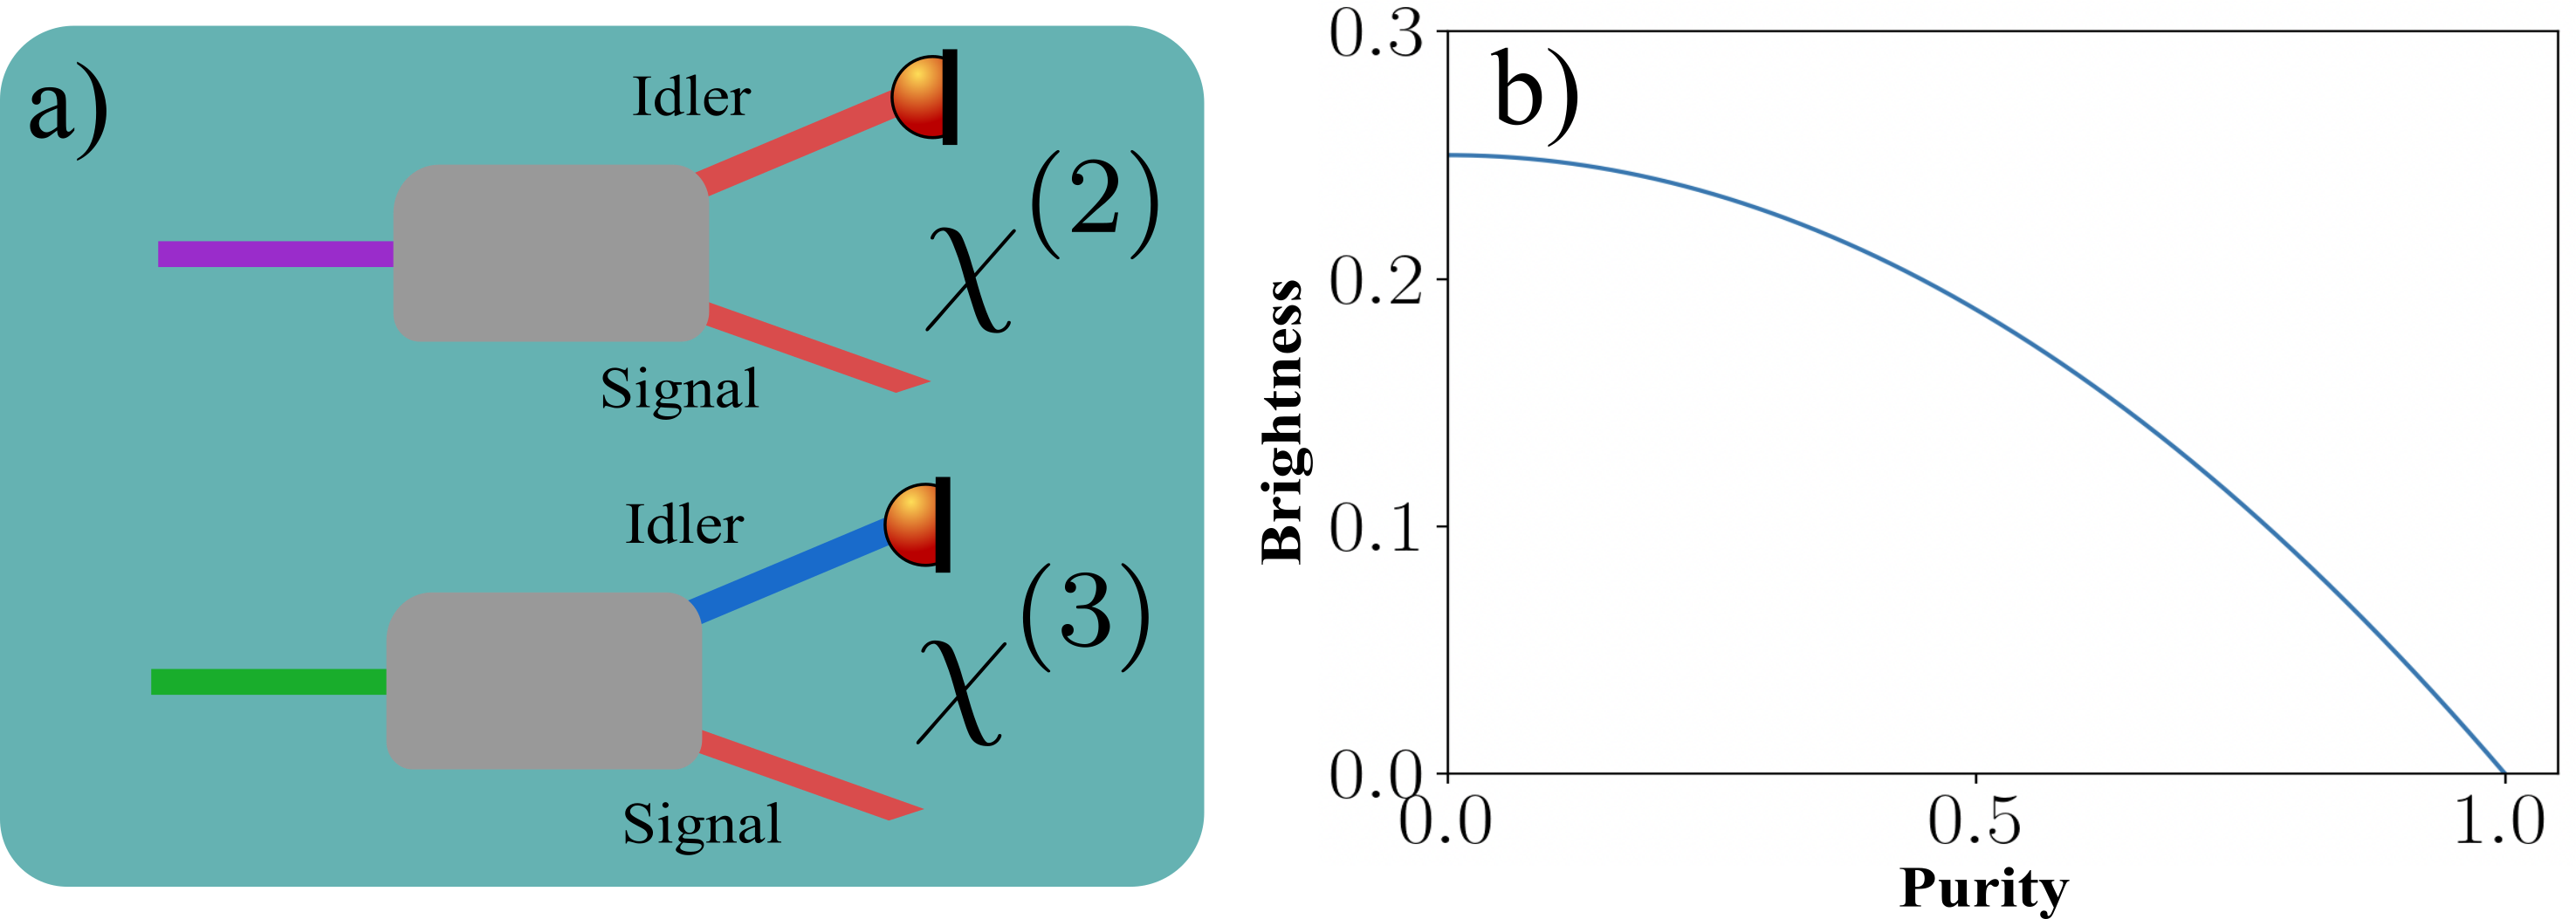
\includegraphics[width=0.9\linewidth]{Figures/SPDC-FWM.png}
    \caption{a) Schematic of $\chi^{(2)}$ and $\chi^{(2)}$, where a pump pulse is converted into two photons. The idler photon is detected yielding the presence of the other signal photon. b) Graphical representation of the trade-off between brightness and purity of probabilistic single-photon sources. The brightness has a maximum of 0.25, at which the purity is 0.}
    \label{fig:SPCD-FWM}
\end{figure}

The quantum state of light emitted from such a source can be modelled as a two-mode squeezed vacuum state \cite{Braunstein2005}:

\begin{equation}
\begin{aligned}
    |\psi\rangle &= \sqrt{1 - |\lambda|^2} \sum_{n=0}^{\infty} \lambda^n  \ket{n}_i\ket{n}_s \\
    &= \sum_{n=0}^{\infty} p_n \ket{n}_i\ket{n}_s,
    \label{eqn:squeezed_state_model}
\end{aligned}
\end{equation}

where $|\lambda|^2 = \tanh^2(r)$ and $r$ is a dimensionless squeezing parameter proportional to the pump laser power \cite{Braunstein2005}. Most setups do not employ photon number resolving detectors and can only register whether any photons are detected, known as `click detectors'. When a detection occurs, the heralded state collapses to a statistical mixture of multi-photon Fock states with $n \geq 1$. The resulting density matrix of the signal mode is given by:

\begin{equation}
    \rho = \sum_{n=1}^{\infty} \frac{|p_n|^2}{\sum_{k=1}^{\infty} |p_k|^2} \ket{n}\bra{n},
    \label{eqn:density_matrix_SPDC}
\end{equation}

The purity of the heralded signal state can be found using a rewritten version of the second-order correlation function, Eqn.~\ref{eqn:g2}:

\begin{equation}
\begin{aligned}
    g^{(2)}(0) &= \frac{\langle \hat{n}(\hat{n} - 1) \rangle}{\langle \hat{n} \rangle^2} \\
    &= \frac{\langle \hat{a}^\dagger \hat{a}^\dagger \hat{a} \hat{a} \rangle}{\langle \hat{a}^\dagger \hat{a} \rangle^2} \\
    &= \frac{\mathrm{Tr}(\rho \hat{a}^\dagger \hat{a}^\dagger \hat{a} \hat{a})}{\left[\mathrm{Tr}(\rho \hat{a}^\dagger \hat{a})\right]^2},
    \label{eqn:g2-tr}
\end{aligned}
\end{equation}

where the number operator $\hat{n}$ has been expressed in terms of the photon creation, $\hat{a}^\dagger$, and annihilation, $\hat{a}$, operators. Eqn.~\ref{eqn:g2-tr} yields $g^{(2)}(0) = 2|\lambda|^2$. Therefore, the purity, as defined in section~\ref{sec:purity}, scales with pump strength as:

\begin{equation}
    P = 1 - 2\tanh^2(r).
\end{equation}

In contrast, the brightness of the source follows the relation:

\begin{equation}
    B = \frac{\tanh^2(r)}{\cosh^2(r)},
\end{equation}

which increases with pump power. This illustrates a fundamental trade-off between brightness and purity in probabilistic sources \cite{Senellart2017}, imposing limitations on the realisation of bright and pure single-photon emission. From Fig.~\ref{fig:SPCD-FWM}b, it can be seen that at the maximum idealised purity, $P=1$, the brightness of the source is 0, and when the brightness is maximised, $B=0.25$, the purity is 0. Recent work has focused on mitigating this limitation by synchronising multiple probabilistic sources within a fast optical switching network to realise an effective deterministic single-photon source \cite{Meyer-Scott2020}. However, this approach requires significant resources and introduces substantial cost and experimental complexity.


\subsubsection{Deterministic Single-photon Sources \label{sec:det-source}}

Deterministic single-photon sources leverage the discrete electronic structure of solid-state emitters, analogous to those found in natural atoms. Typically, a laser pulse is used to excite the emitter from its ground state to a higher-energy excited state. A single photon is then emitted during the spontaneous relaxation back to the ground state \cite{Weisskopf1930}, enabling controlled and on-demand photon generation.

However, in solid-state systems, these emitters are embedded within a surrounding lattice, which introduces non-radiative decay channels such as vibrations. These mechanisms compete with radiative relaxation, which reduces both the emission efficiency and the indistinguishability of the emitted photons. The total decay rate of solid-state sources can be expressed as the sum of radiative and non-radiative contributions: $\gamma = \gamma_{\mathrm{rad}} + \gamma_{\mathrm{nrad}}$. The impact of non-radiative processes is characterised by the quantum efficiency, $\eta_{\mathrm{QE}}$, defined as:

\begin{equation}
    \eta_{\mathrm{QE}} = \frac{\gamma_{\mathrm{rad}}}{\gamma_{\mathrm{rad}} + \gamma_{\mathrm{nrad}}}.
    \label{eqn:qe}
\end{equation}

To experimentally determine quantum efficiency, a method introduced by Drexhage is often used \cite{Tews1970, Drexhage1968}. By varying the distance between the emitter and a mirror, the local optical density of states—and thus $\gamma_{\mathrm{rad}}$—is modified, while $\gamma_{\mathrm{nrad}}$ remains unchanged. Measuring how the total decay rate varies with emitter–mirror separation enables extraction of the quantum efficiency.


Recent advances in solid-state single-photon sources have focused on improving purity, stability, and importantly, scalability. Self-assembled quantum dots (QDs) are the benchmark for single-photon emission but require cryogenic conditions. Monolayer transition metal dichalcogenides (TMDCs), such as WSe$_2$, offer strong exciton binding energies and atomically thin structures but also operate at low temperatures. In contrast, hexagonal boron nitride (hBN), with its wide ~6 eV bandgap, chemical stability, and ability to emit at room and cryogenic temperatures, is an attractive candidate for practical quantum technologies. Table~\ref{tab:emitter-comparison} summarises $g^{(2)}(0)$ values for each emitter, with QDs showing the highest purity.


\begin{table}[h]
\centering
\begin{tabular}{|c|c|c|}
\hline
\textbf{Emitter} & \textbf{Reported $\mathbf{g^{(2)}(0)}$} & \textbf{Operating Temperature} \\
\hline
QDs & $<0.02$ \cite{Hanschke2018, Heiss2013} & Cryogenic  \\
\hline
TMDCs & $\sim0.05 $ \cite{Parto2021, Piccinini2025} & Cryogenic  \\
\hline
hBN & $<0.1$ \cite{Vogl2021, Xu2018}  & Cryogenic \\
\hline
hBN & $<0.1$ \cite{Zeng2022, Grosso2017, Vogl2017} & Room Temperature \\
\hline
\end{tabular}
\caption{Comparison of solid-state single-photon emitters}
\label{tab:emitter-comparison}
\end{table}


\subsection{\label{sec:source_prep}hBN Preparation: Fabrication and Excitation}

\subsubsection{Fabrication Methods}

hBN consists of Boron and Nitrogen atoms arranged in a 2D hexagonal lattice, Fig.~\ref{fig:struc}a. Within each atomic layer, atoms are bonded by strong covalent interactions, while adjacent layers are held together by weaker van der Waals forces. This structure results in a wide bandgap of approximately 6~eV, making it suitable for hosting point defects that can act as stable sources of single photons, \cite{Tran2016, Cholsuk2024}.

\begin{figure}[h]
    \centering
    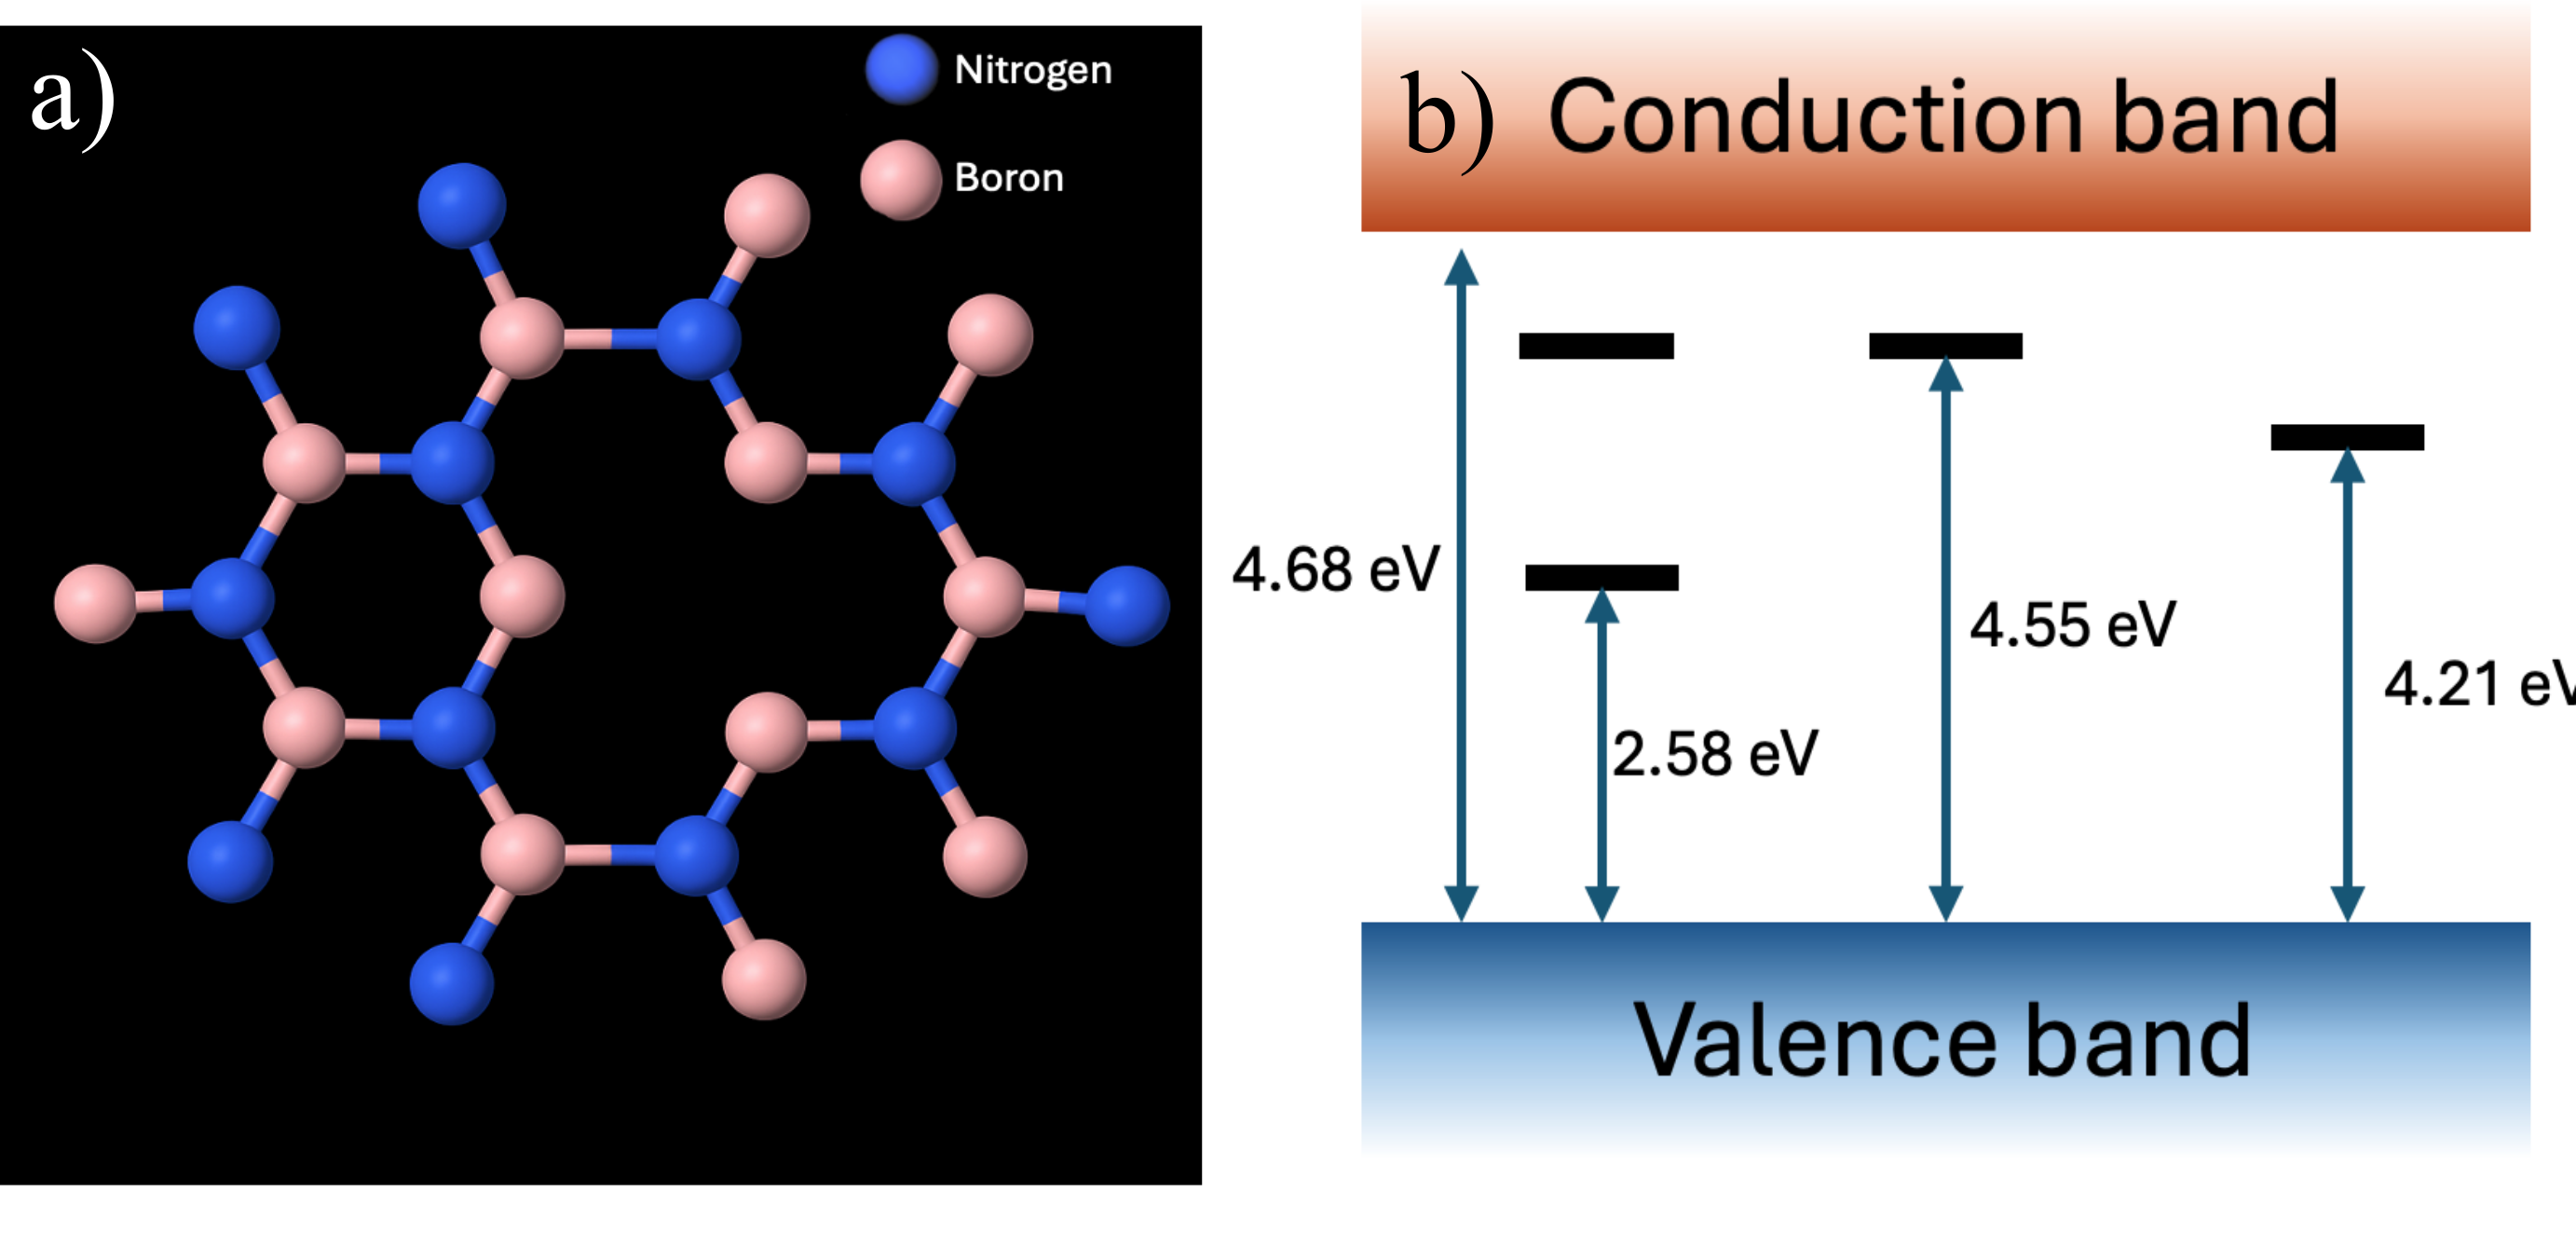
\includegraphics[width=0.9\linewidth]{Figures/hBNStructure.png}
    \caption{a) Atomic structure of hBN, showing a nitrogen vacancy defect. Nitrogen atoms are shown in blue and boron atoms in pink. b) Electronic energy levels associated with a nitrogen vacancy in hBN. Defect levels form within the bandgap and give rise to characteristic optical transitions \cite{Tran2016}.}
    \label{fig:struc}
\end{figure}


hBN can host both naturally occurring and artificially induced defect centres, commonly referred to as colour centres. Natural defects can be stabilised and activated through annealing \cite{Mohajerani2024}, while artificial defects can be induced via electron beam irradiation. Such irradiation techniques have been shown to produce single-photon emitters with emission centred around 532~nm following thermal annealing \cite{NgocMyDuong2018, Bianco2023}. The precise mechanisms by which colour centres are formed is not fully understood, and a comprehensive classification of the various possible defect types is still ongoing. To support this effort, several databases are being developed to catalogue known and predicted defect configurations, employing machine learning and density functional theory techniques to guide identification and analysis \cite{Cholsuk2024, zotero-item-9536}. An example of the molecular structure of a Nitrogen vacancy defect, and the resulting energy level structure can be seen in Fig.~\ref{fig:struc}.

Both naturally occurring and electron beam-induced defect formation methods were explored, but samples subjected to electron irradiation did not yield detectable emission, likely because the excitation laser wavelength was lower in energy than the typical emission energies of such defects. Various hBN samples were tested under different annealing conditions with mixed success, summarised in Table~\ref{hBN-creation}. The most successful sample was provided by Serkan Ateş’s group at the İzmir Institute of Technology, Turkey, containing naturally occurring defects that exhibited bright, stable emission without additional processing. This sample was drop-cast onto a distributed Bragg reflector (DBR) mirror with 10 alternating SiO$_2$ and TiO$_2$ layers, reflecting light by constructive interference from the refractive index contrast (see Appendix for reflectivity data). All results presented in this work were obtained from this sample.



\begin{table}[h]
    \centering
    \small
    \begin{tabular}{|c|p{3.9cm}|p{2.7cm}|p{5.4cm}|}
        \hline
        \textbf{Batch} & \textbf{Properties} & \textbf{Source} & \textbf{Comments} \\
        \hline
        A & Annealed in nitrogen and argon; commercial dissolution & Graphene\newline  Supermarket & Some bright defects found between 575–590~nm, but rare and hard to locate. \\
        \hline
        B & Annealed in argon; commercial dissolution & Graphene\newline  Supermarket & Emitters were unstable and disappeared after a few seconds. \\
        \hline
        C & Annealed in argon; powder dissolved in acetone & Graphene\newline  Supermarket & Noisy but bright emitters around 575~nm. High flake density made them easy to find. \\
        \hline
        D & Annealed in nitrogen; powder dissolved in acetone & Graphene\newline  Supermarket & Weak spectral features around 575~nm and 630~nm. Overall emission was faint and noisy. \\
        \hline
        E & Annealed in hydrogen and argon; powder dissolved in acetone & Graphene \newline Supermarket & Poor spectral quality with weak, noisy features. \\
        \hline
        F & Solution drop-cast on DBR mirror & İzmir Institute of Technology & Bright, stable emitters across a broad spectral range. Most successful sample. \\
        \hline
    \end{tabular}
    \caption{Overview of tested hBN samples and annealing outcomes.}
    \label{hBN-creation}
\end{table}


\subsubsection{Excitation Schemes}

The emission spectrum of a solid-state emitter comprises the zero-phonon line (ZPL) and the phonon sideband (PSB). The ZPL is a higher-energy, prominent feature corresponding to purely radiative transitions from the excited to the ground state without phonon involvement, while the PSB appears as a broader, lower-energy component arising from radiative relaxation to a vibrational sublevel followed by non-radiative phonon emission. This work focuses on the non-resonant excitation of hBN defects, where the emitter is pumped with a laser of higher energy than the ZPL. This approach simplifies filtering via long-pass filters and avoids the need for a tunable laser but introduces drawbacks, including timing jitter and increased dephasing that degrade photon indistinguishability, as well as the risk of simultaneously exciting other defects, reducing photon purity.

Alternative excitation schemes include resonant excitation, which requires tuning the laser precisely to the ZPL, and quasi-resonant excitation, where the laser is scanned across the ZPL. In practice, resonant driving often results in collecting PSB photons due to easier separation from the excitation light, but both methods necessitate tunable lasers not available in this work. Another consideration is the choice between pulsed and continuous wave (CW) excitation; pulsed excitation is crucial for quantum technologies because it enables precise timing control necessary for quantum communication and computation. In this work, both excitation modes are used according to the requirements of each measurement.


\subsection{Comparative Analysis of Solid-State Emitter Properties}

\subsubsection{\label{sec:coherence-time} Coherence Time}

The timescale over which an emitter produces indistinguishable photons is known as the coherence time, $T_2$, and is given by:

\begin{equation}
    \frac{2}{T_2}=\Gamma/2\pi=\gamma/2\pi+2\gamma^*/2\pi
\end{equation}

where $\gamma$ is the spontaneous decay rate of the emitter and $\gamma^*$ is the pure dephasing rate. The full width at half maximum, $\Gamma/2\pi$, of an emitter’s spectrum is related to its coherence time by $\Gamma/2\pi=2/T_2$. In the absence of pure dephasing ($\gamma^*=0$), the emitter is Fourier transform-limited, with a linewidth determined solely by the spontaneous emission rate ($\Gamma=\gamma$), emitting perfectly indistinguishable photons without any loss during emission. Although such Fourier-limited linewidths have been demonstrated using quasi-resonant excitation \cite{Dietrich2018}, this ideal scenario is rarely realised under other excitation schemes due to spectral wandering and phonon-induced dephasing.

At low temperatures, where phonon interactions are suppressed, the ZPL often shows inhomogeneous broadening caused by slow spectral diffusion from local electric field fluctuations \cite{Sontheimer2017}, producing a Gaussian-like lineshape. Spectral diffusion has been observed to increase with excitation power, especially near saturation \cite{White2021}. As the temperature increases, colour centres like those studied here exhibit spectral broadening from phonon interactions, with dephasing scaling as $\Gamma \propto T^5$ \cite{Ari2025}, consistent with strong electron–phonon coupling.

The indistinguishability of a source can be calculated by $I= T_2/(2T_1)=\gamma/\Gamma$. Values for indistinguishability vary significantly across solid-state emitter platforms, table~\ref{tab:t2-compare}.

\begin{table}[h]
\centering
\begin{tabular}{|c|c|c|}
\hline
\textbf{Emitter} & \textbf{Reported $I$} & \textbf{Operating Temperature} \\
\hline
QDs & $>0.95$ \cite{Ulhaq2010, Somaschi2016} & Cryogenic  \\
\hline
TMDCs & $0.003$ \cite{vonHelversen2023} & Cryogenic  \\
\hline
hBN & $0.2-0.4$ \cite{Fournier2023, Horder2022}  & Cryogenic \\
\hline
\end{tabular}
\caption{Comparison of solid-state single-photon emitter indistinguishability}
\label{tab:t2-compare}
\end{table}


\subsubsection{Quantum Efficiency and Debye-Waller Factor}

Although the coherence time of an emitter is the most important factor when considering its suitability for use in quantum technologies which rely on photon entanglement, other numerical quantities such as the quantum efficiency, Eqn.~\ref{eqn:qe} and Debye-Waller $DW$ factor should be taken into account. The $DW$, quantifies the fraction of photons emitted without phonon coupling, and is defines as:

\begin{equation}
    DW=\frac{I_{ZPL}}{I_{TOTAL}},
\end{equation}

where $I_{ZPL}$ and $I_{TOTAL}$ is the intensity of the ZPL and ZPL+PSB spectrum, respectively. It is critical for a single-photon emitter to maximise both the $\eta_{\text{QE}}$ and $DW$ factor. Therefore, it is important to consider the product of these, $\eta = \eta_{\text{QE}}\times DW$, when considering the suitability of a source. It can be seen in Table~\ref{tab:eta-compare} that all emitters discussed in section~\ref{sec:det-source} exhibit relatively high values of $\eta$:

\begin{table}[h]
\centering
\begin{tabular}{|c|c|c|}
\hline
\textbf{Emitter} & $\mathbf{\eta}$ & \textbf{Operating Temperature} \\
\hline
QDs & $\sim0.7$ \cite{Somaschi2016} & Cryogenic  \\
\hline
TMDCs & $\sim0.2$ \cite{Micevic2022,Cai2024} & Cryogenic  \\
\hline
hBN & $\sim0.3$ \cite{Tran2016, Yamamura2024} & Cryogenic \\
\hline
\end{tabular}
\caption{Comparison of solid-state single-photon emitter $\eta = \eta_{\text{QE}} \times DW$}.
\label{tab:eta-compare}
\end{table}
